\documentclass[12pt,a4paper]{article}
\usepackage[
type={CC},
modifier={by-nd},
version={4.0},
]{doclicense}
\usepackage[utf8]{inputenc}
\usepackage[T1]{fontenc}
\usepackage{amsmath}
\usepackage{amssymb}
\usepackage{graphicx}
\usepackage[french]{babel}
\usepackage[a4paper]{geometry}
\geometry{top=20mm,bottom=15mm,inner=15mm,outer=10mm}
\DeclareUnicodeCharacter{000B}{}
\usepackage{listings}
\usepackage{color}
\usepackage{float}

\definecolor{codegreen}{rgb}{0,0.6,0}
\definecolor{codegray}{rgb}{0.5,0.5,0.5}
\definecolor{codepurple}{rgb}{0.58,0,0.82}
\definecolor{backcolour}{rgb}{0.95,0.95,0.92}

\lstdefinestyle{mystyle}{
    backgroundcolor=\color{backcolour},
    commentstyle=\color{codegreen},
    keywordstyle=\color{magenta},
    numberstyle=\tiny\color{codegray},
    stringstyle=\color{codepurple},
    basicstyle=\ttfamily\footnotesize,
    breaklines=true,
    numbers=left,
    numbersep=5pt,
    tabsize=2
}
\lstset{style=mystyle}

\setlength{\parskip}{0.2em}
\newcommand{\rep}[1]{\fbox{$#1$}}

\title{Rapport 1 -- Soundway Groupe 3 \\ \mbox{ } \\
Projet à réaliser dans le cadre du cours \\
INFO M435 -- Interfaces incarnées et augmentées}
\author{Esteban BARRACHO\\
        Anas DAMLAKHI\\
        Jonathan KONDOLI NKEBI\\
        Arthur SMOOS\\
        Bénédicte TUTEKA MUKUTA\\
Faculté d'informatique, Université de Namur}
\date{Année académique 2025-2026}

\begin{document}
\maketitle
\thispagestyle{empty}
\vspace*{13em}

\begin{figure}[H]
    \centering
    
\includegraphics[width=0.3\textwidth]{LogoUNamur.jpg}
    \label{fig:LogoUNamur}
\end{figure}

\pagebreak

\section{Introduction}

Le projet SoundWay vise à développer un système d’aide à l’orientation reposant sur des balises Bluetooth (BLE), un backend capable d’interpréter la distance, et une application mobile intuitive. L’objectif est d’aider une personne à se déplacer autour de la Faculté d’informatique via un guidage assisté et une reconnaissance vocale simple d’usage.

Ce rapport présente la réflexion de départ, les choix techniques majeurs, un exemple de code minimal, les écrans de l’application, ainsi que les difficultés rencontrées lors de la construction du prototype.

\section{Réflexion sur la conceptualisation}

Dès le début, nous avons conçu SoundWay comme un système modulaire composé de trois éléments :

\begin{itemize}
    \item un \textbf{émetteur BLE} (Raspberry Pi),
    \item un \textbf{récepteur BLE} (smartphone),
    \item une \textbf{interface mobile} qui affiche l’information utile.
\end{itemize}

Le Bluetooth s’est révélé sensible aux variations et aux pertes de paquets. Un seul signal n’était pas suffisant pour obtenir une distance stable. Grâce à l’application nRF Connect, nous avons remarqué que plusieurs advertisements simultanés amélioraient la fluidité. Nous avons donc adopté un modèle multi-advertisements, tous sous le même nom \texttt{King375}.

Ce choix était simple à mettre en œuvre et améliorait réellement la qualité des mesures.

\subsection{Exemple de Code : Émetteur BLE et Récepteur}

\textbf{Émetteur BLE (Raspberry Pi) -- Pseudocode} :

\begin{lstlisting}[language=Txt]
connecter au bus DBus système
charger l'interface Bluetooth (BlueZ)

définir les paramètres BLE (intervalle min/max)

pour i = 0 à 4 :
    créer une annonce BLE
    enregistrer l'annonce
    afficher "Annonce active"

boucle infinie :
    attendre
\end{lstlisting}

\textbf{Récepteur BLE (Bleak) -- Pseudocode} :

\begin{lstlisting}[language=Txt]
démarrer le scanner BLE

lorsqu'un signal BLE est reçu :
    si le nom est "King375" :
        afficher l'adresse et la puissance du signal

boucle infinie :
    attendre
\end{lstlisting}


\newpage

\section{Interface mobile développée}

En parallèle du travail Bluetooth, nous avons conçu l'application mobile SoundWay. Les fonctionnalités essentielles sont déjà opérationnelles, notamment la reconnaissance vocale.

\subsection{Écrans d'acceuil et d’authentification}

\begin{figure}[H]
    \centering
    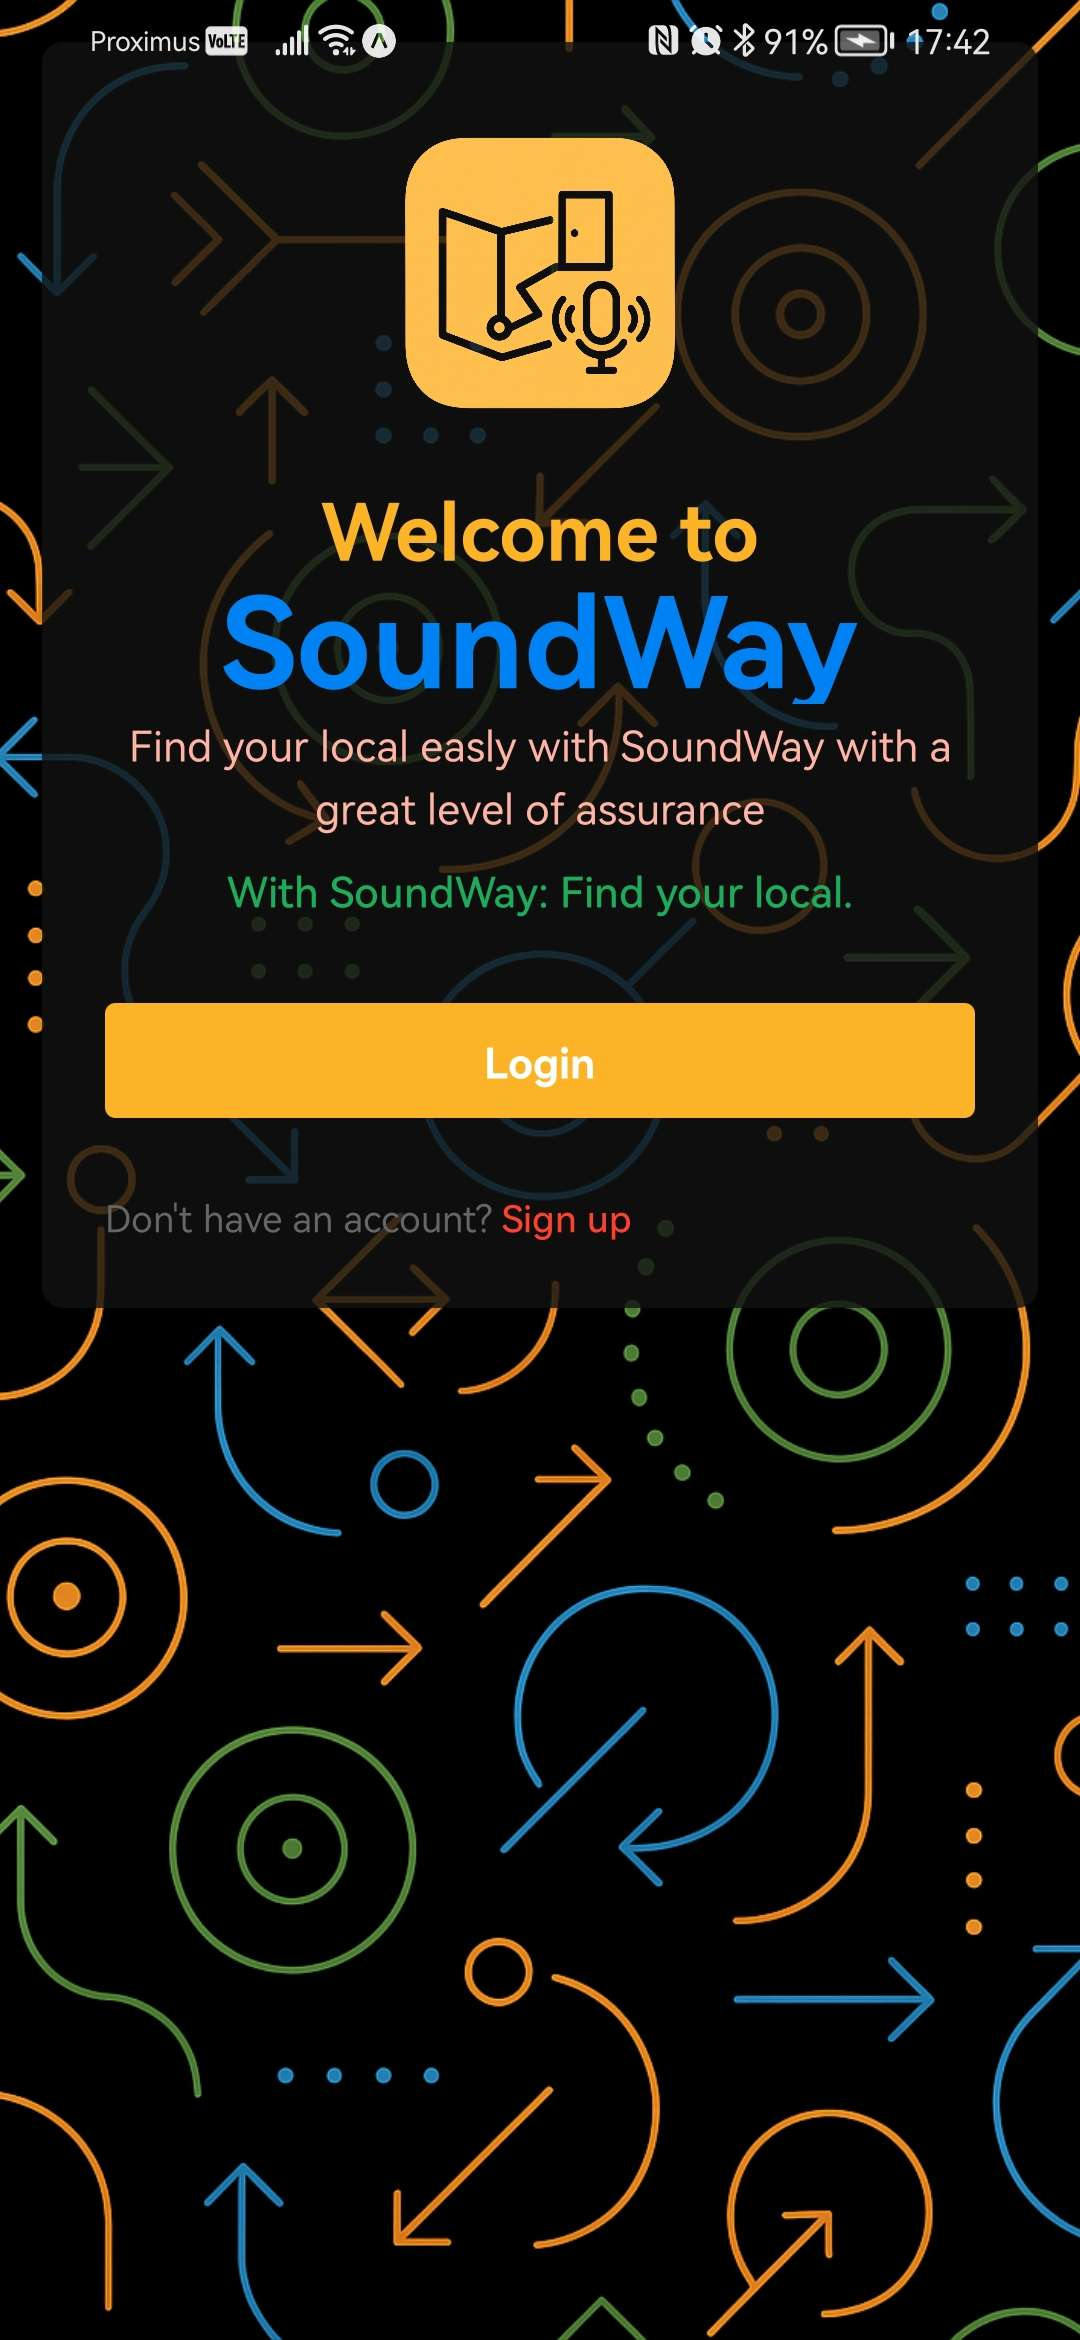
\includegraphics[width=0.25\textwidth]{2025-11-06 – SoudWay-App-1.jpg}
    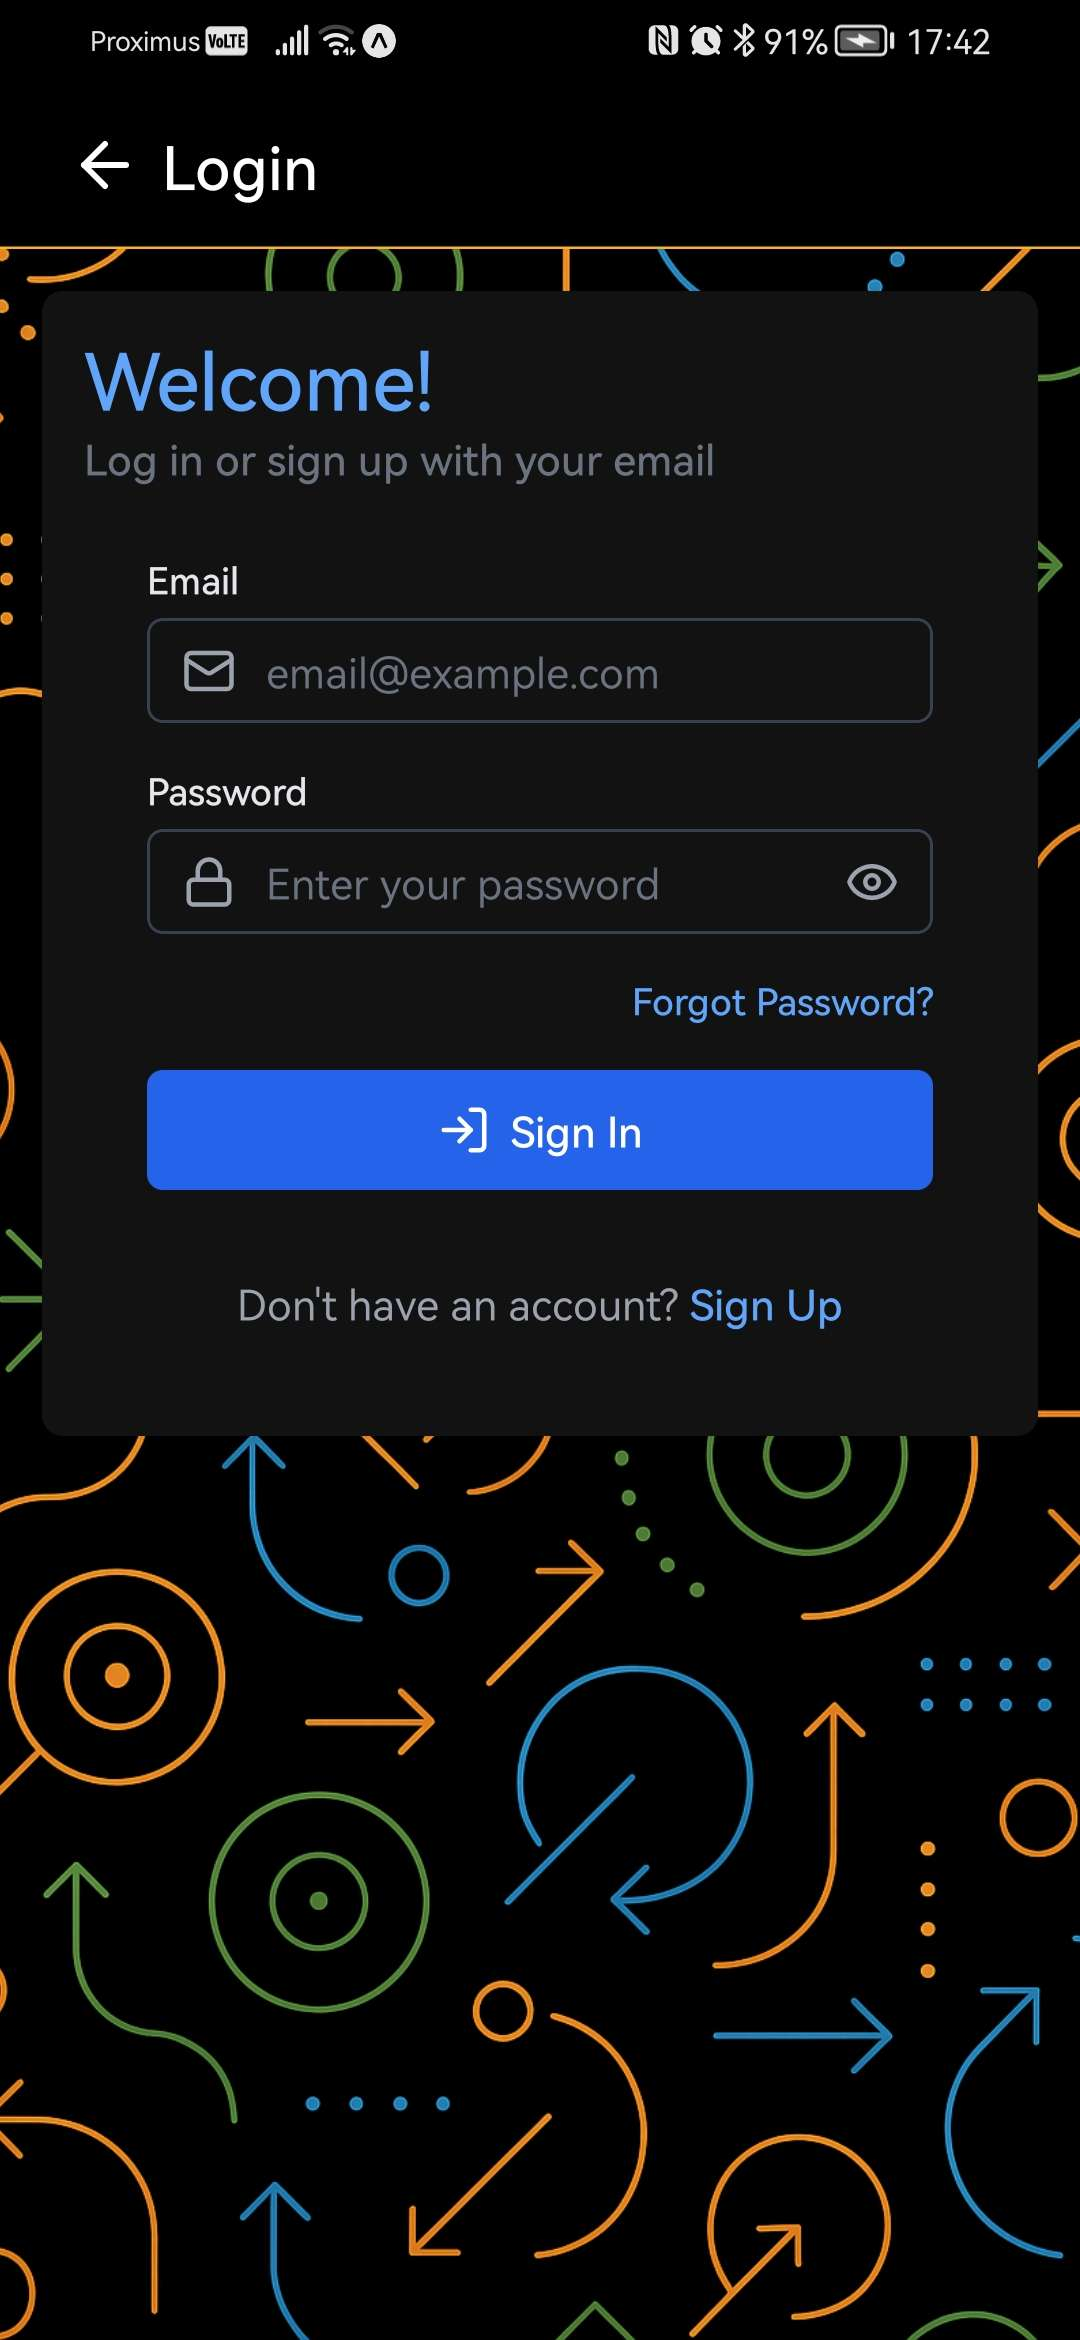
\includegraphics[width=0.25\textwidth]{2025-11-06 – SoudWay-App-2.jpg}
    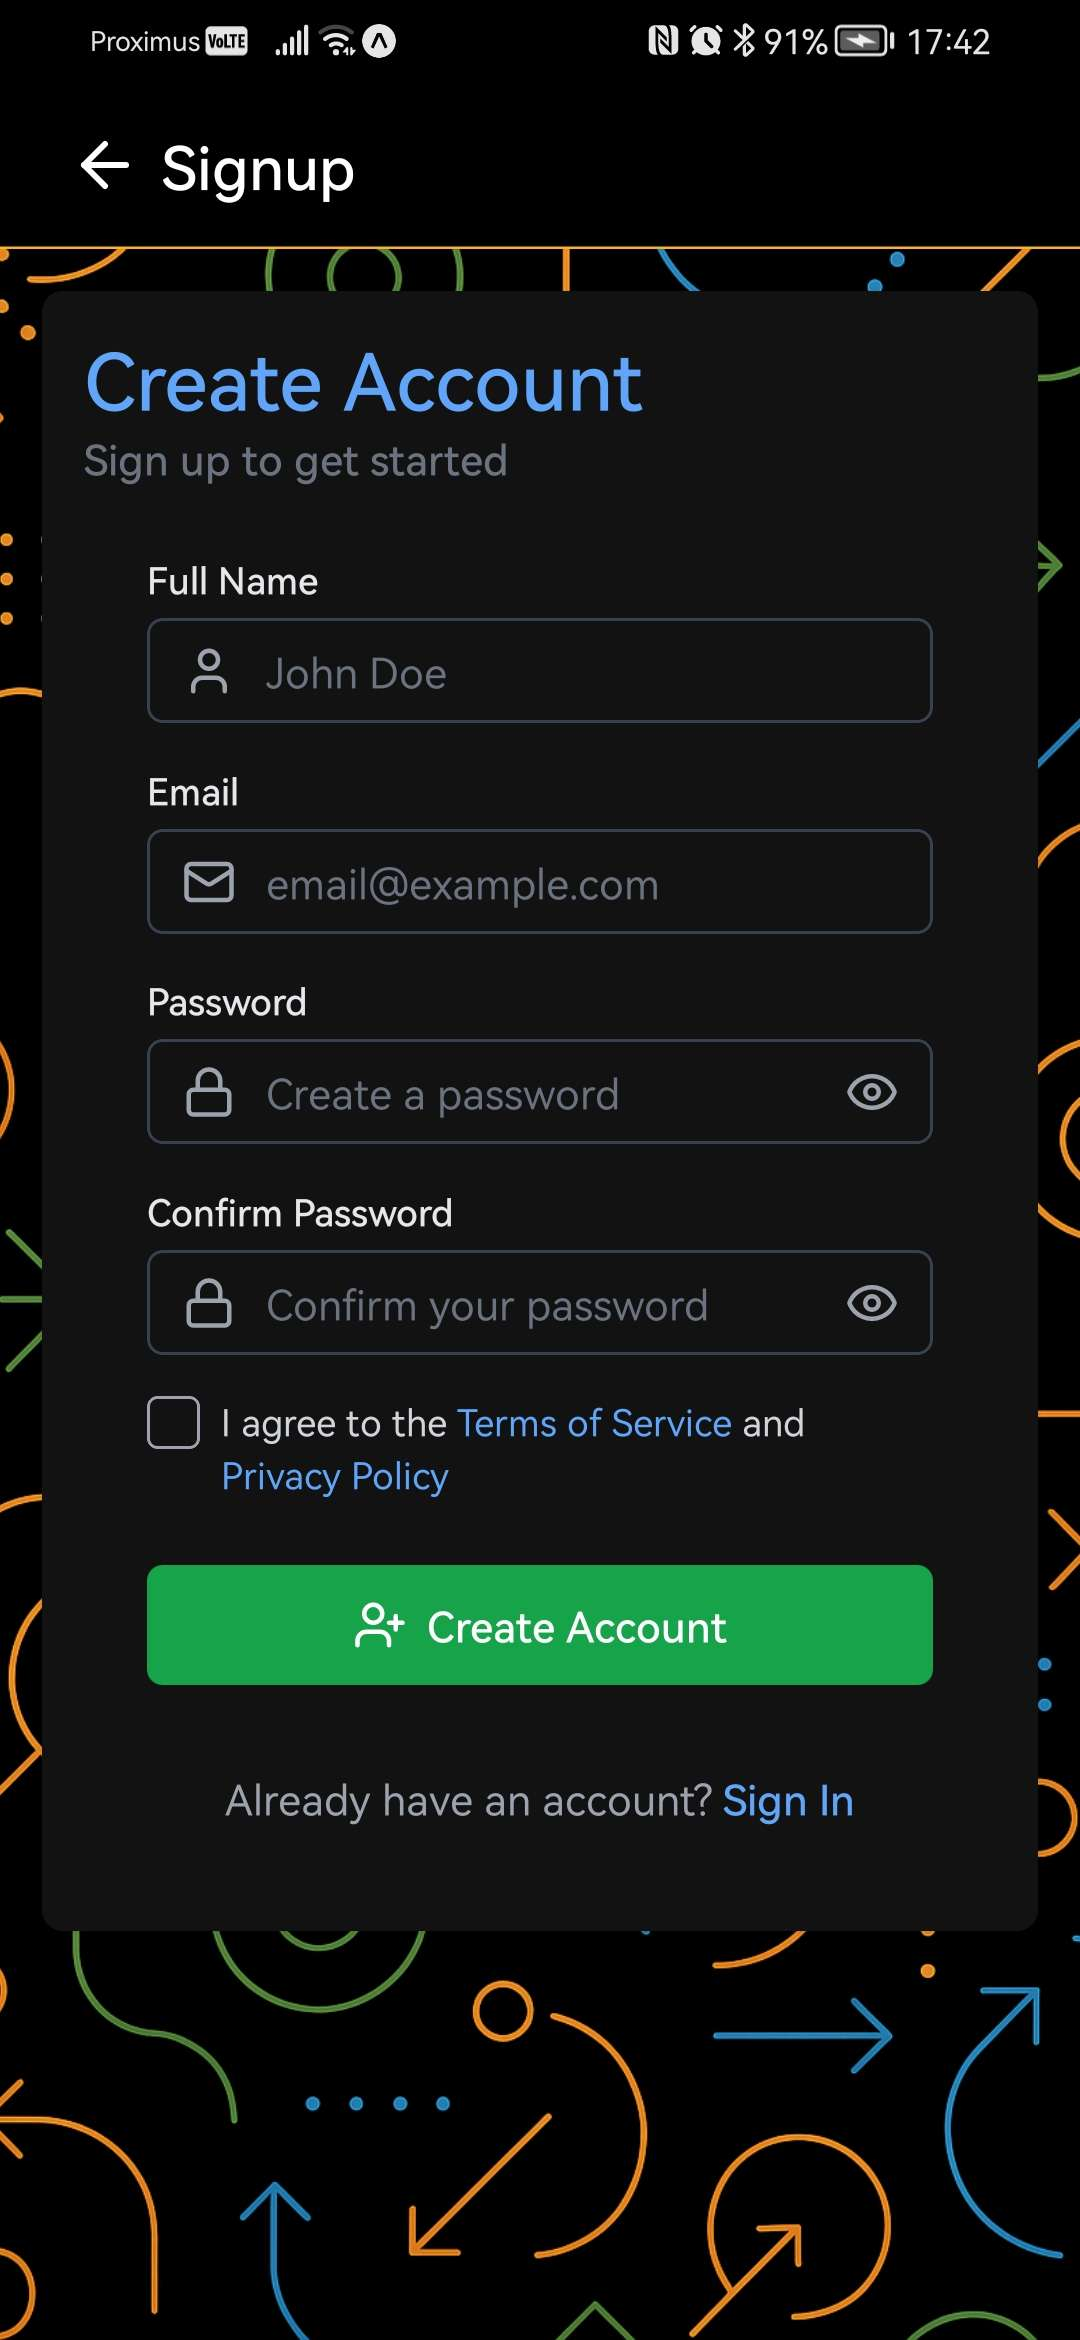
\includegraphics[width=0.25\textwidth]{2025-11-06 – SoudWay-App-3.jpg}
    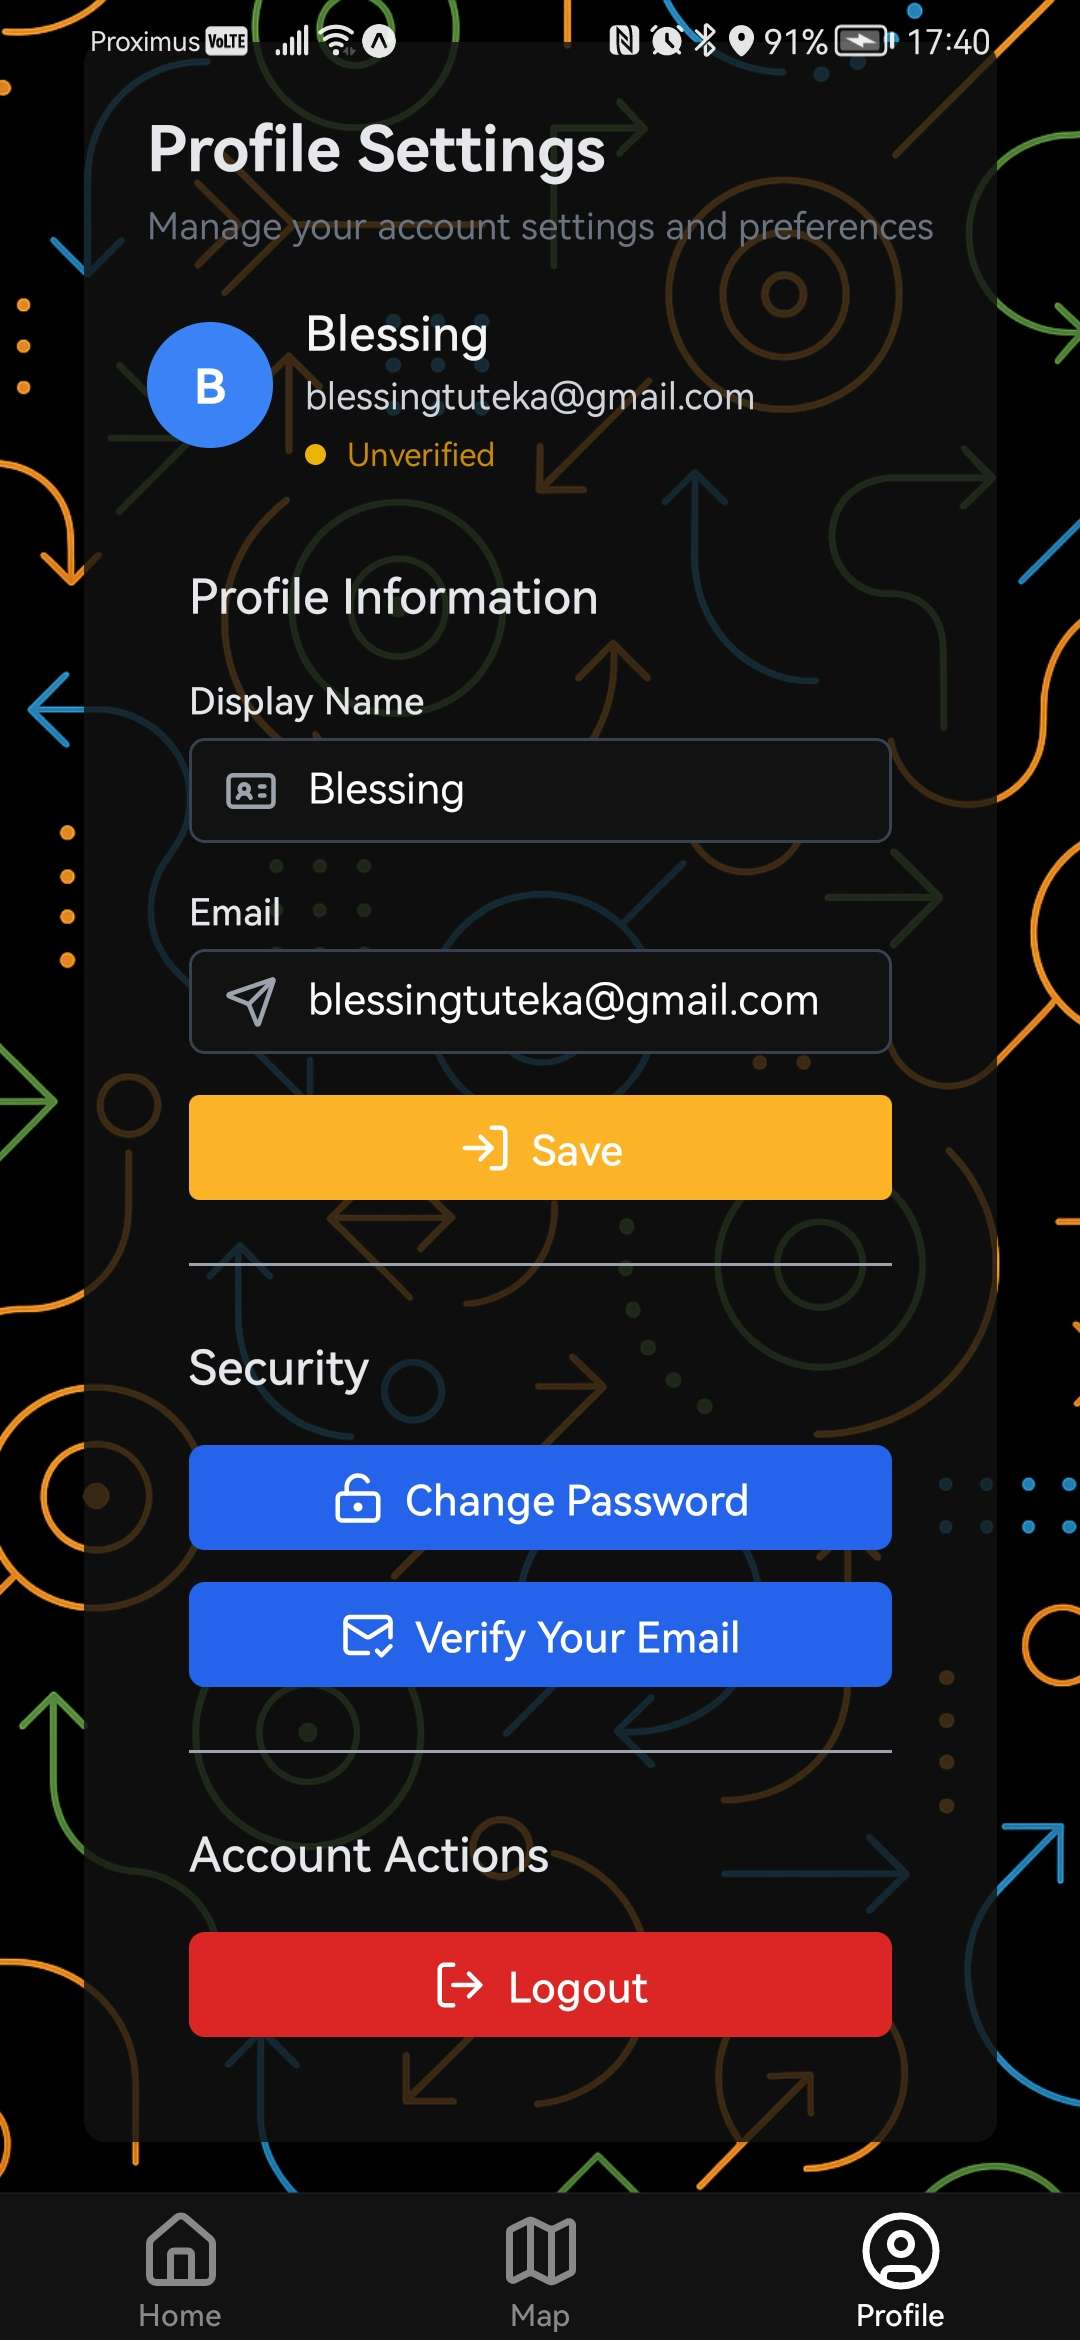
\includegraphics[width=0.25\textwidth]{2025-11-06 – SoudWay-App-6.jpg}
    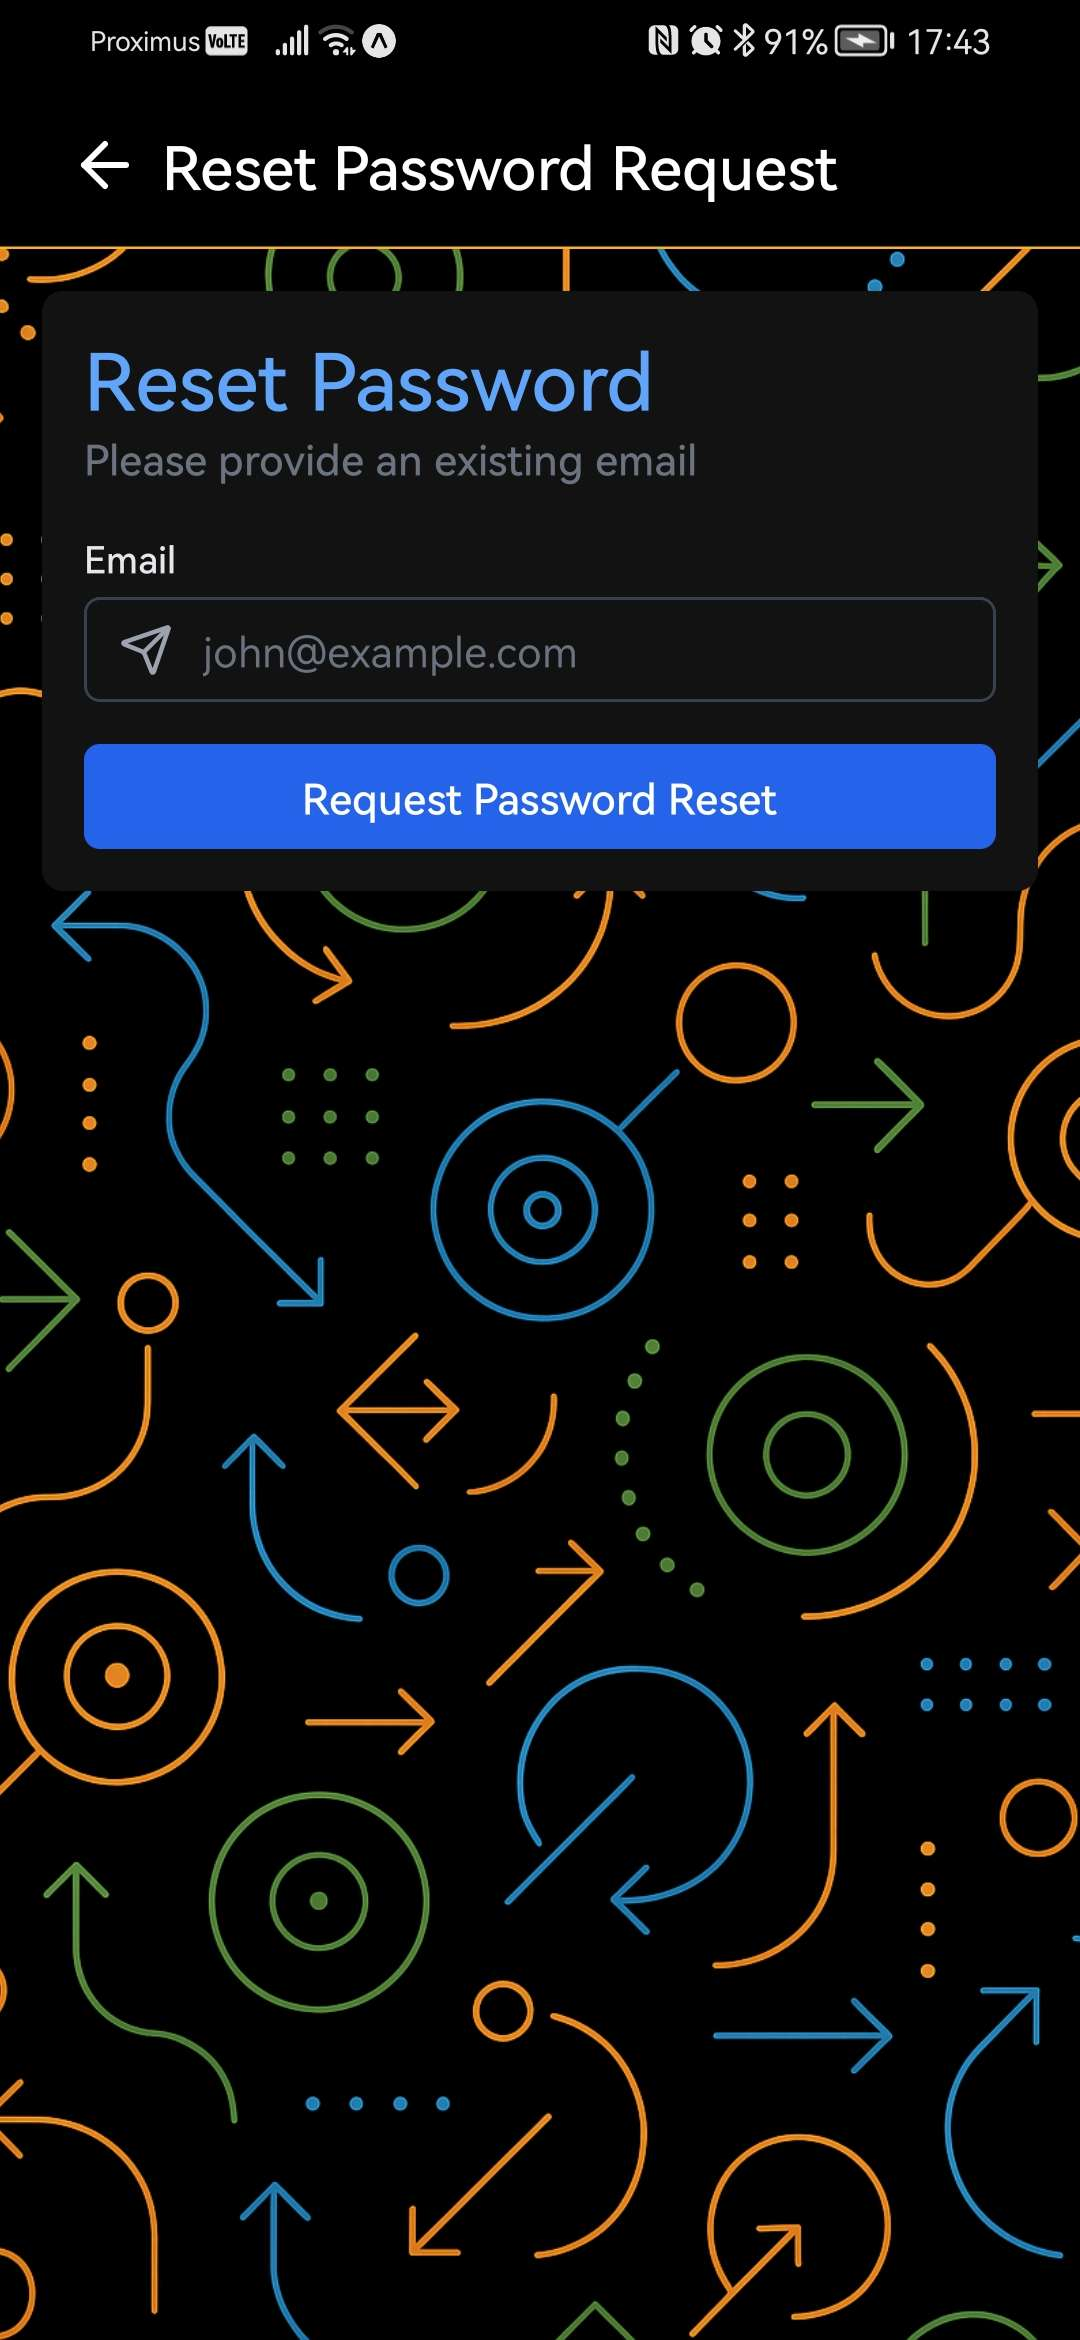
\includegraphics[width=0.25\textwidth]{2025-11-06 – SoudWay-App-4.jpg}
    \caption{Login, création de compte et modifiation, réinitialisation du mot de passe}
    
\end{figure}

\subsection{Reconnaissance vocale et Direction}

\begin{figure}[H]
    \centering
    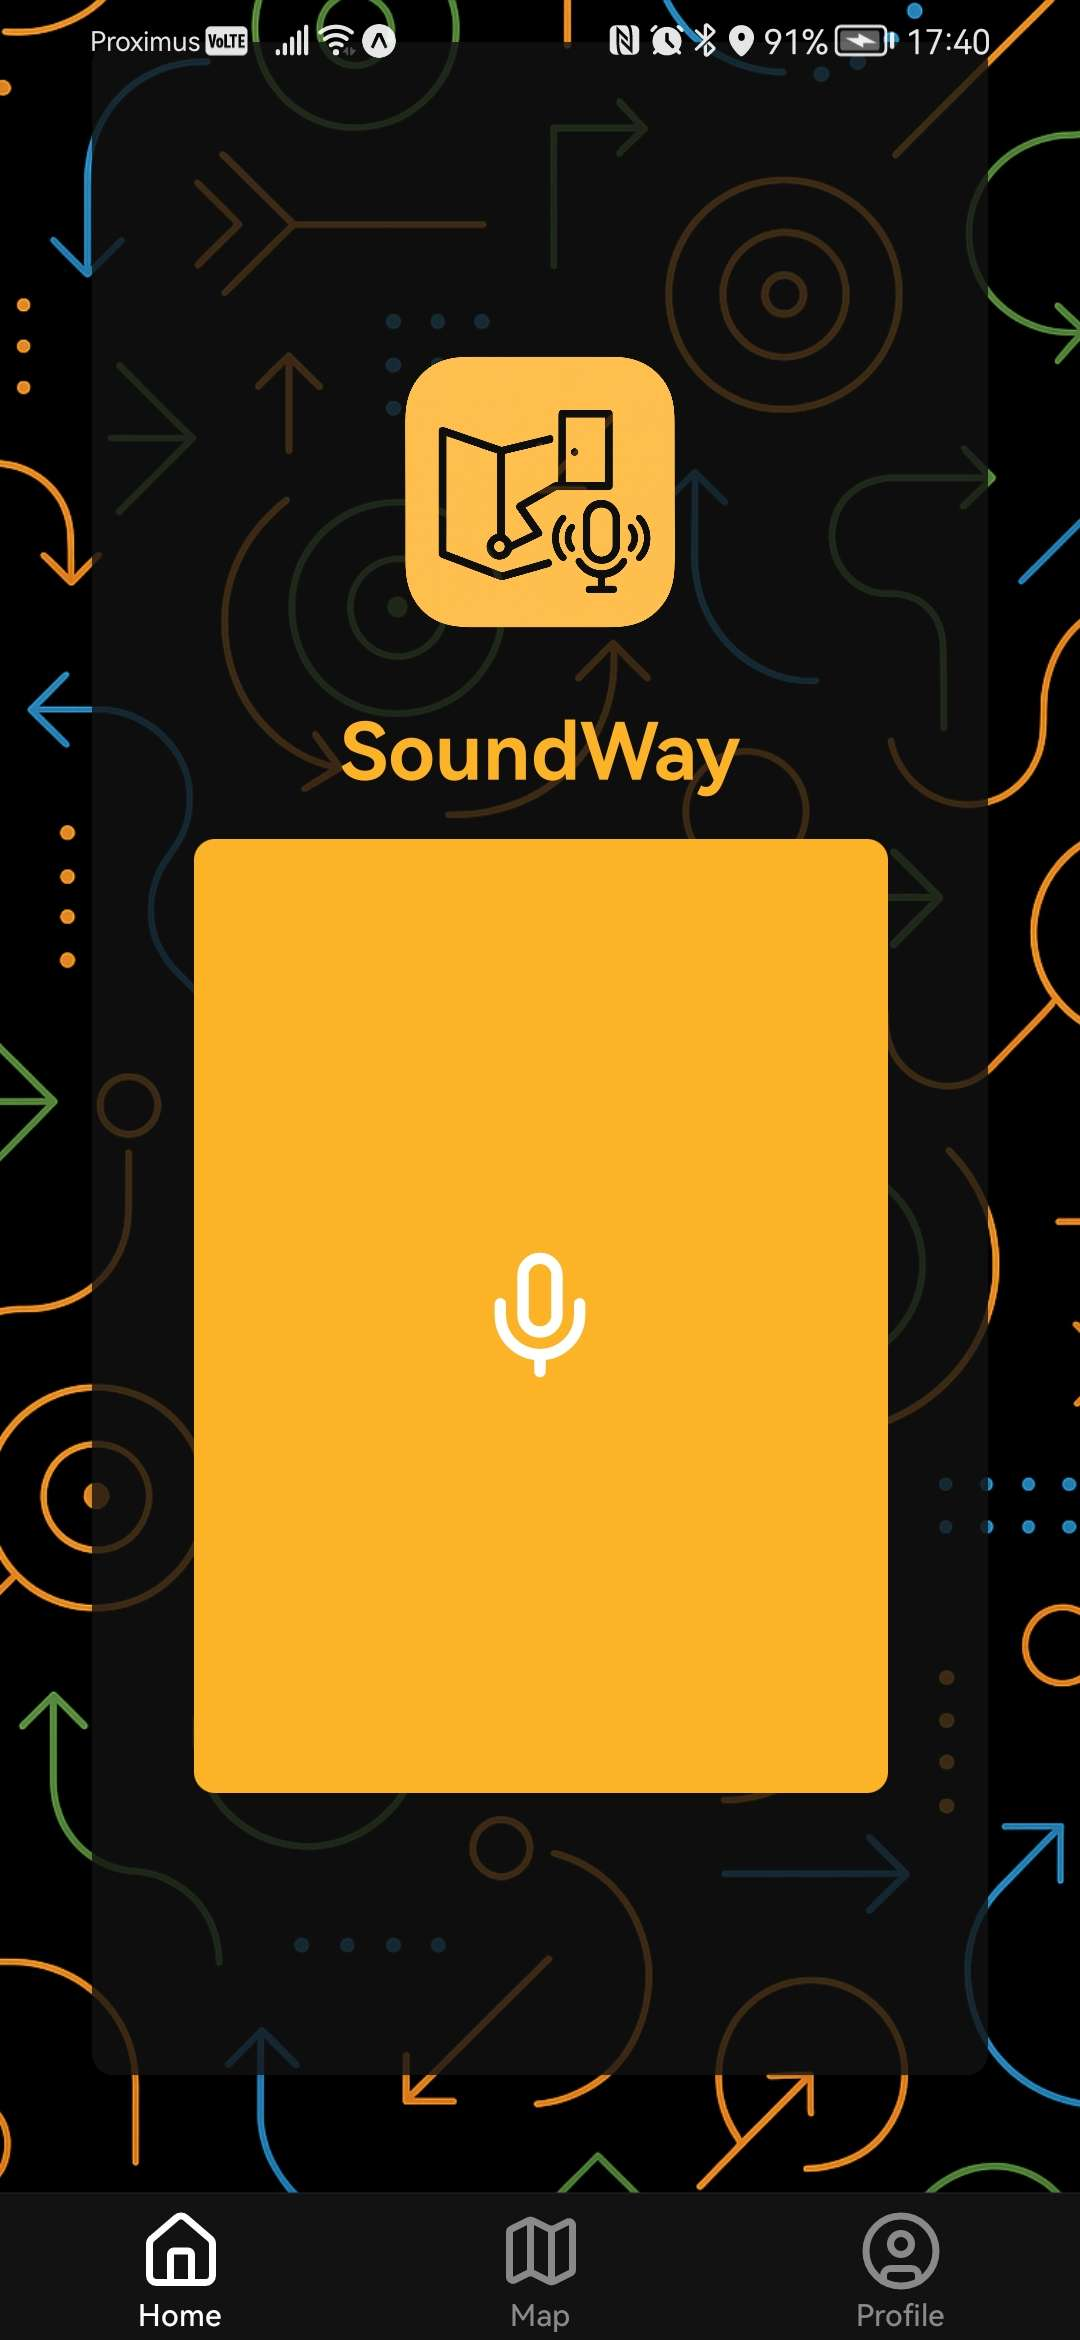
\includegraphics[width=0.25\textwidth]{2025-11-06 – SoudWay-App-5.jpg}
    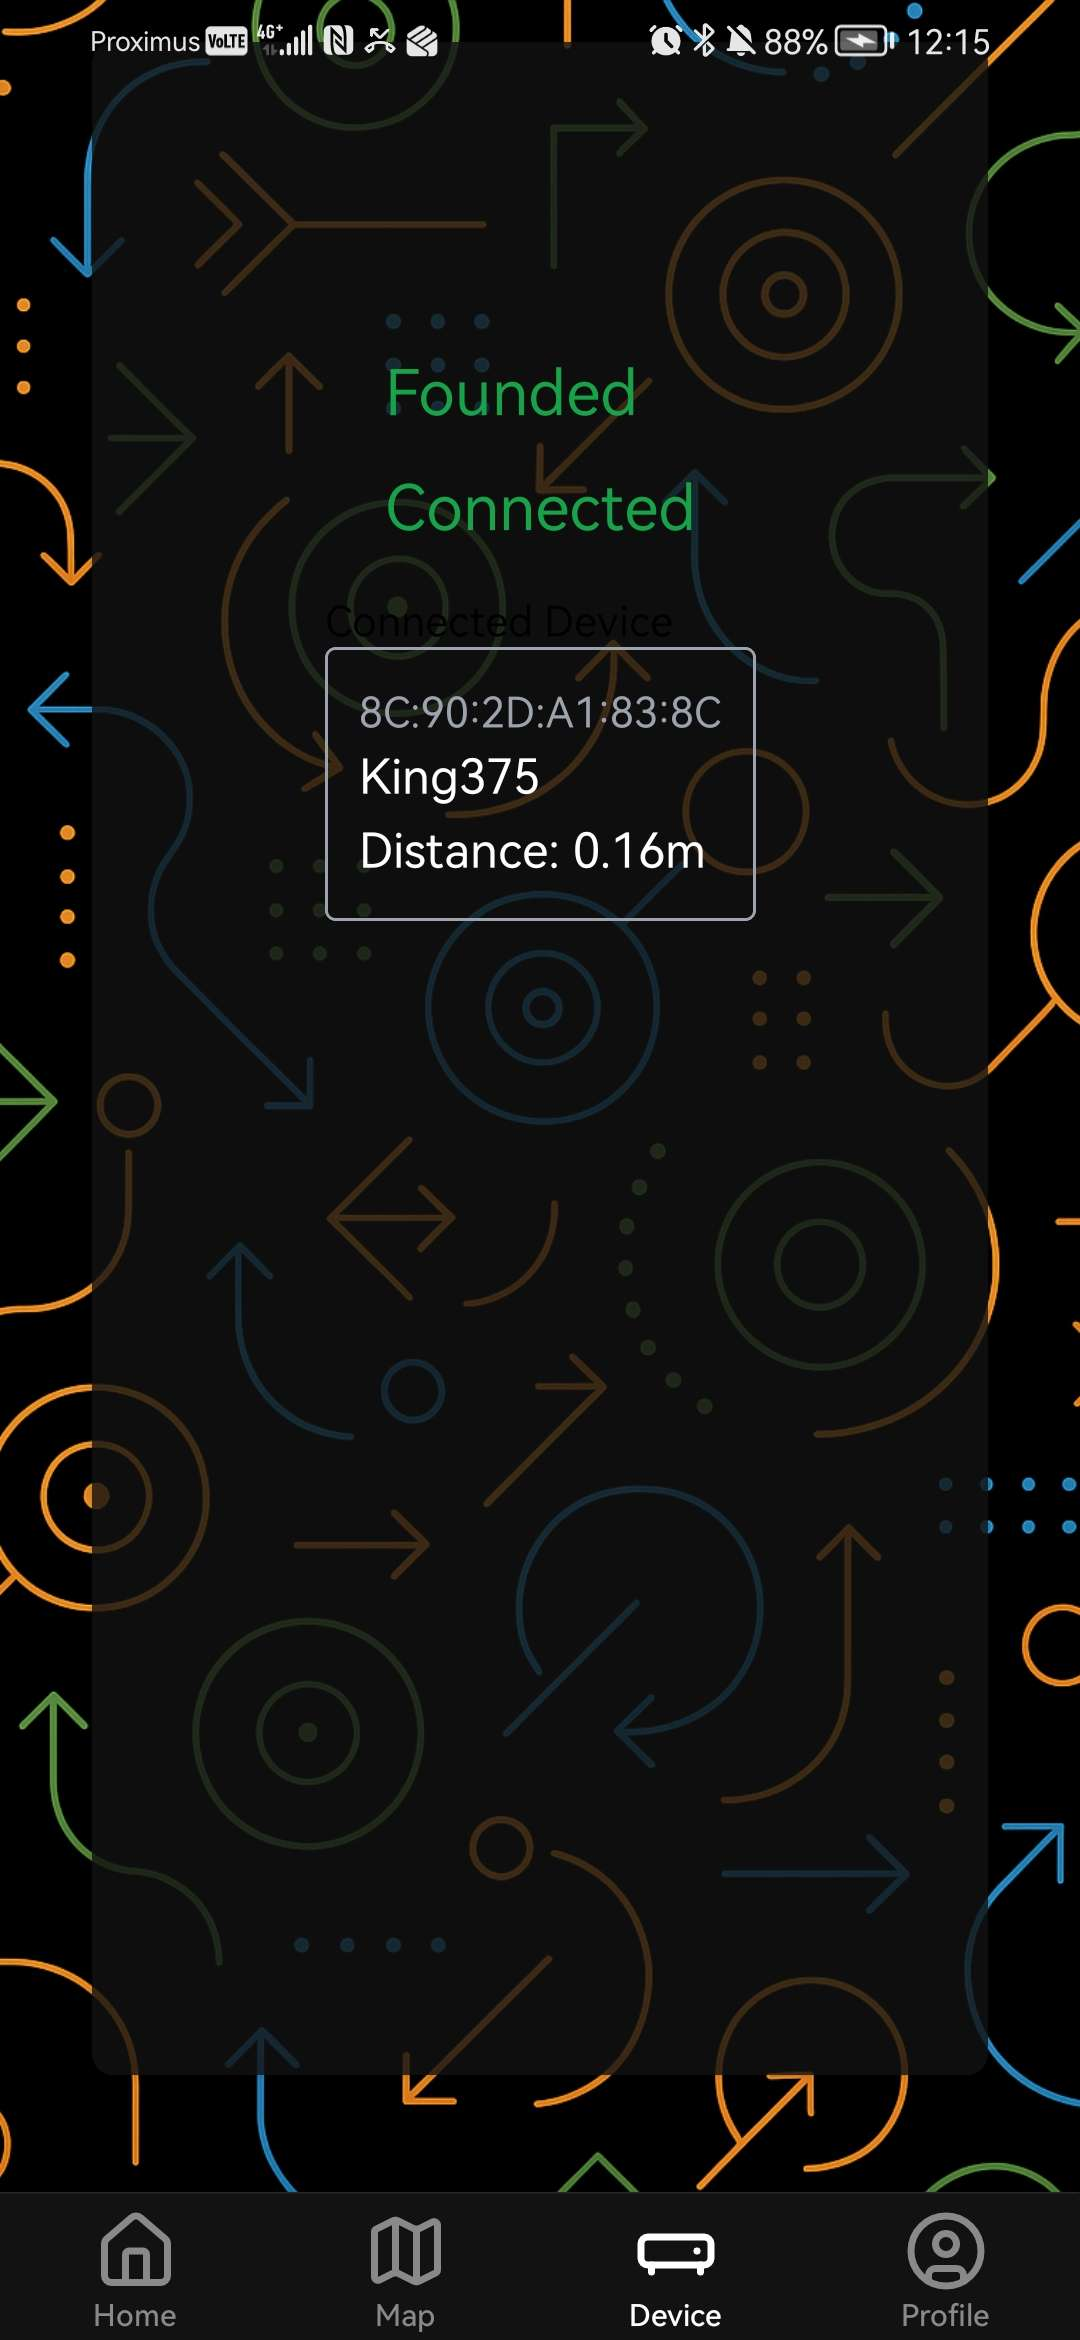
\includegraphics[width=0.25\textwidth]{2025-11-18 – SoudWay-App-8.jpg}
    \caption{Écran – microphone et distance}
\end{figure}

\subsection{Carte et navigation}

\begin{figure}[H]
    \centering
    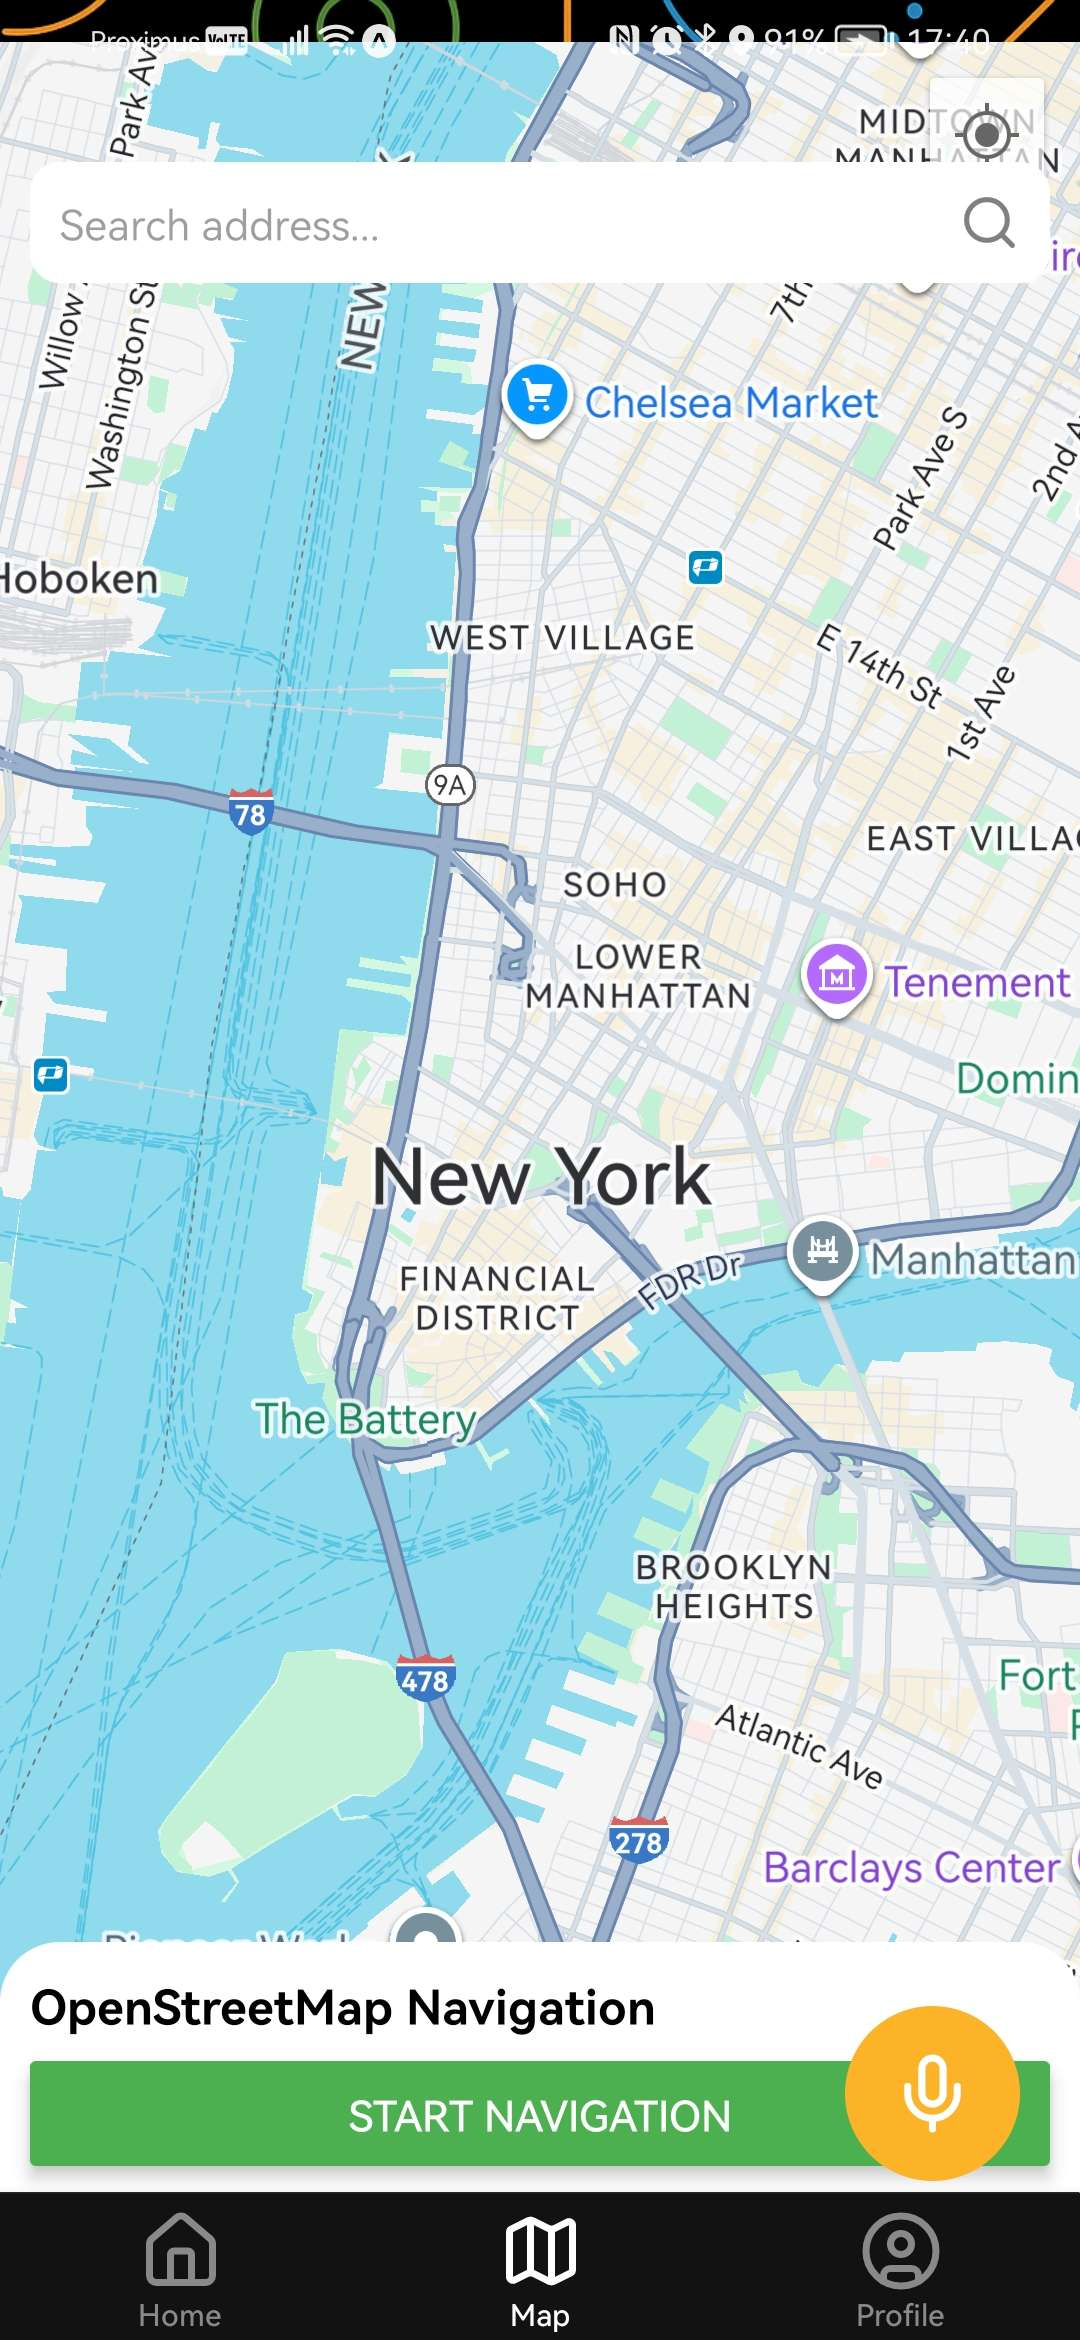
\includegraphics[width=0.25\textwidth]{2025-11-06 – SoudWay-App-7.jpg}
    \caption{Carte OpenStreetMap intégrée}
\end{figure}

\section{Marche à suivre}

\begin{itemize}
    \item Mise en place des advertisements BLE.
    \item Calibration du \texttt{tx\_power}.
    \item Agrégation et filtrage des signaux.
    \item Développement des écrans mobiles.
    \item Intégration de la reconnaissance vocale.
\end{itemize}

\section{Problèmes rencontrés}

\begin{itemize}
    \item Premier Raspberry défectueux : aucun Bluetooth.
    \item Peu d'expérience mobile pour une partie du groupe.
    \item Problèmes de rafraîchissement.
    \item Suppression de la map car nécessite un achat clé API
\end{itemize}

\section{Résolution}

\begin{itemize}
    \item Nouveau Raspberry + clé USB Bluetooth.
    \item Documentation et aide entre membres.
    \item Correction progressive en ce basant sur les réponses front-end obtenue et aujourd’hui stable et fonctionnel grâce à une fonction callback.
\end{itemize}

\section{Conclusion}

Nous avons obtenu un prototype complet : un backend fiable, une application mobile fonctionnelle avec reconnaissance vococale, et un système BLE multi-advertisements précis et robuste. La suite consistera à connecter les deux mondes et tester SoundWay en conditions réelles autour de la faculté.

\bigskip
\hrule
\bigskip

{\small \noindent © 2025 Esteban BARRACHO.\\
Ce document est distribué selon la licence Creative Commons CC BY-ND.
\doclicenseThis}

\bigskip
\hrule
\end{document}
